\documentclass{jsarticle}
\usepackage{nitkc-senkoka-chukan}
% 日本語フォント設定
\usepackage[deluxe, jis2004]{otf}
\usepackage{pxchfon}
\usepackage{graphicx}
\setmediumminchofont{HaranoAjiMincho-Medium.otf} % \mcfamily\mdseries
\setboldminchofont{HaranoAjiMincho-Bold.otf} % \mcfamily\bfseries
\setmediumgothicfont{HaranoAjiGothic-Medium.otf} % \gtfamily\mdseries
\setboldgothicfont{HaranoAjiGothic-Bold.otf} % \gtfamily\bfseries


\title{企画・中間発表会フォーマット}
\author{武市 ~半平太}
\affiliate{竜馬研究室}
\keywords{キーワード1,キーワード2,Keyword3}

\begin{document}

\maketitle

\section{はじめに}
このフォーマットは,卒業研究における企画・中間発表会の要約集に関する,電気情報工学科の統一フォーマットです.{\LaTeX}で書いていただけることを想定しています.これらの形式に慣れることで,これから将来,皆さんが学会投稿などをするときに戸惑わないような期待もあります.
なお,このフォーマットは皆さんでより良いものにしていくものです.是非アイデアやご意見をお寄せください.

{\LaTeX}の基本操作や環境設定,書きかたなどは多くの参考書\cite{total}\cite{latex}\cite{okumura},Web情報がありますのでそちらをご覧ください.

\section{利用方法}
原稿作成に当たってはA4判白紙に,以下の体裁に従って内容の記載・図表の添付を行います.この説明書をよくお読みになった上で原稿をお書き下さい.

\subsection{作成上の注意}
別途配布している{\LaTeX}のテンプレートを利用すれば,各種書式とフォントは自動的に設定されます.

\begin{enumerate}
  \item A4判白紙に,原稿執筆見本に示す体裁(この原稿出力結果)に従って内容の記載・図表の添付を行います.
  \item 上下左右のマージンおよび講演番号スペースを確保します.マージンは上マージン25mm,左マージン20mm,カラム間マージン5mm,右マージン20mm,下マージン25mmを目安としてレイアウトに留意して下さい.
  \item 印刷時はカラー写真は白黒になります.
  \item 使用言語は,日本語または英語
  \item 配置
\begin{itemize}
  \item 	表題,著者名,所属は原稿執筆見本に従い,記入して下さい.表題,著者名が1ページ目の最上部,勤務先が1ページ目の左下部に位置します.英文の場合は,表題のみ英文で記入して下さい.
  \item 	本文は1段または2段に書いても差支えありません.
\end{itemize}
  \item 表題,著者名,所属,本文の文字の大きさは,下記を大体の目安として下さい.
\begin{itemize}
  \item 	表題 12ポイント
  \item 	著者名・勤務先 10.5ポイント
  \item 	本文見出し 10.5ポイント
  \item 	本文 9ポイント
\end{itemize}
\end{enumerate}

\subsection{見出し}

節や小節の見出しには \verb|\section|, \verb|\subsection| といったコマンドを使用する.
\verb|\section|の見出しは2行を占め,他は1行に出力される.

\subsection{文章の記述}

\begin{description}
\item[文体]
「ですます調」ではなく,「である調」で記述すること.平易な文体でありながら,丁寧且つ論理的な文章作りに努めること.

\item[句読点]
句点には全角の「.」,読点には全角の「,」を用いる.ただし英文中や数式
中で「.」や「,」を使う場合には,半角文字を使う.「。」や「、」は一切使
わない.

\item[全角文字と半角文字]
全角文字と半角文字の両方にある文字は文章全体で統一して使い分けること.
例えば,括弧は全角の「(」と「)」を用いる,但し,英文の概要,図表見出し,書誌
データでは半角の「(」と「)」を用いる,などとすると良い.
\end{description}

%図を挿入する場合は以下の%を外してコピーして使ってください

%\begin{figure}[hbtp]
%\begin{center}
%\resizebox{8cm}{!}{\includegraphics{feistel.eps}}
%%上の「8cm」と書いてある所は図の横幅です.適宜変更してください.
%%ただし最大が8cmとなっています.
%\caption{図のタイトル}
%\label{ラベル名}
%\end{center}
%\end{figure}

% 図の挿入
\begin{figure}[tb]
  \begin{center}
    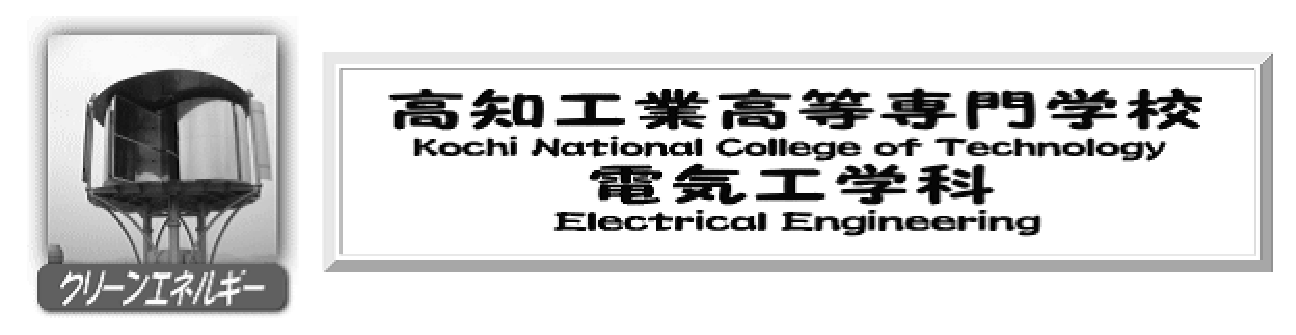
\includegraphics[keepaspectratio=true,height=.20\hsize]{KNCT-EE.eps}
  \end{center}
  \caption{図の例}%{}内にタイトルを記入してください
  \label{KNCT-EE}
\end{figure}

\begin{table}[tb] \caption{表の例}
\label{tab:table-env}
% 左右の罫線はつけず,一番上の罫線は二重線
\hbox to\hsize{\hfil
\begin{tabular}{l|cc}\hline\hline
&Server&Viewer\\\hline
CPU&P2-450MHz&P3-850MHz\\
Memory&256MB&384MB\\
OS& \multicolumn{2}{|c}{WindowsXP-ProfessionalSP1}\\
Interface& \multicolumn{2}{|c}{IEEE802.3(10Mbps)}\\
& \multicolumn{2}{|c}{IEEE802.3u(100Mbps)}\\\hline
\end{tabular}\hfil}
\end{table}

\subsection{図}
図\ref{KNCT-EE}のように図も挿入できます.
2段の幅にまたがる図も描けます.

\subsection{表}
勿論,表\ref{tab:table-env}のように表も書けます.
表の罫線はなるべく少なくするのが,仕上がりをすっきりさせるコツです.罫線を
つける場合には,一番上の罫線には二重線を使い,左右の端には縦の罫線をつけない方が良いとされます.

\subsection{数式}
どんな数式も大丈夫です.
\begin{eqnarray}
\lefteqn{ \int\!\!\!\int_S 
 \left(\frac{\partial V}{\partial x}
 -\frac{\partial U}{\partial y}\right)
 dxdy} \quad\nonumber\\
 &=& \oint_C \left(U{dx \over ds}
      + V{dy \over ds}\right)ds
\end{eqnarray}
\\
\begin{equation}
 \def\quad{\hskip.75em\relax}
 %% デフォルトは \hskip1em
 A = \pmatrix{
      a_{11} & a_{12} & \ldots & a_{1n} \cr
      a_{21} & a_{22} & \ldots & a_{2n} \cr
      \vdots & \vdots & \ddots & \vdots \cr
      a_{m1} & a_{m2} & \ldots & a_{mn} \cr
     }
\end{equation}

\section{参考文献リスト}
参考文献リストには,原則として本文中で引用した文献のみを列挙する.順序は参照
順あるいは第一著者の苗字のアルファベット順が良い.

\section{PDFファイル作成上の注意}
上記に加えてPDFファイル作成上で以下のような注意点があります.
\begin{enumerate}
  \item ファイルサイズ(容量)の制限 \\
ファイルサイズは,制限しませんが,余りにも大きくなる場合はサーバにUPLOADする前に相談してください.またファイルは各資料ごとに一つとし,圧縮ツールによる圧縮やセキュリティ設定はしないでください.
  \item 使用できるフォントの制限 \\
PDFファイルは,Windows及びMacintosh対応にするため,原稿内に使用するフォントは以下に限定してください.これ以外のフォントを使用されると,利用する環境によっては文字化けを起こすことがあります.
\\
使用可能な日本語フォント
\begin{itemize}
  \item Windows:MS明朝またはMSゴシック
  \item Macintosh:細明朝または中ゴシック
  \item 平成明朝または平成角ゴシック
  \item 使用可能な英語フォント:Arial,Century,Times, Times New Roman, Helvetica, Symbol
\end{itemize}
またコンピュータの機種により文字化けが発生する可能性がありますので,漢字コードは第二水準以内の文字をお使いください.特にMacintosh をお使いの方はローマ数字や丸付き数字などの特殊記号については必ずJISコードをご利用ください.

  \item 色使い \\
文字も含め,色使いの制限は特にありません.ただしモノクロプリンタで出力したものを論文集の原稿として利用しますので,色によっては明確に出ない場合がありますので十分注意してください.
  \item 写真や画像などの解像度 \\
写真や画像を含む場合,PDF化することにより,出力品質が劣化することがあります.ファイルサイズ制限内で,PDF化する際のジョブオプションの値を高くして作成してください.Distillerを使う場合は,Imageの圧縮をAutoではなく,ZIPにすると解像度が向上します.
  \item ファイル形式 \\
電子原稿は,Adobe Acrobat Reader4.0以上で表示または印刷可能なPDF(Portable Document Format)ファイルで提出してください.
  \item ファイル名について \\
必ず拡張子(.pdf)がついているファイルをお送りください.
  \item 作成するアプリケーションとOS \\
原稿を作成するアプリケーションの制限はありません.OSはWindows95以上またはMacintosh 7.5以上を推奨します.
  \item PDFファイルの作成方法 \\
{\LaTeX}とDviout,Ghostscriptなどを使っている場合は,いくつかのフリーツールによってPDFファイルが作成できます.dvipdfm(x)などが良いでしょう.

商用ソフトを利用する場合は,原則としてAcrobat 4.0以降(または同等品)を用いて作成します.作成方法については付属のマニュアルまたはWEB上の作成方法をご覧ください.
Acrobat の詳細についてはhttp://www.adobe.co.jpをご覧ください.また必ずAcrobat Distillerを使って作成してください.特にイラストや画像,数式,グラフ等を含むPDFファイルの作成はPDF Writerを使用しないでください.

\end{enumerate}


\begin{thebibliography}{99}
\bibitem{total}
伊藤和人: {\LaTeX} トータルガイド, 秀和システムトレーディング (1991).

\bibitem{latex}
Lamport, L.: {\em A Document Preparation System {\LaTeX} User's Guide \&
  Reference Manual\/}, Addison Wesley, Reading, Massachusetts (1986).
\newblock (Cooke, E., et al.訳:文書処理システム {\LaTeX},アスキー出版局
  (1990)).

\bibitem{okumura}
奥村晴彦: 改訂第3版{\LaTeX2e} 美文書作成入門, 技術評論社 (2003).

\end{thebibliography}

\end{document}
